\section{Introduction à la CAO \& à l'impression 3D}

\subsection{Qu'est-ce que la CAO ?}

\begin{flushleft}
    La CAO, ou Conception Assistée par Ordinateur (Computer Aided Design en anglais) est l'ensemble des logiciels et des techniques de modélisation géométriques permettant de simuler et de visualiser la structure et le fonctionnement d'un objet en prévision de sa fabrication. De nos jours elle est couramment utilisée dans l'industrie.\\
    Il existe de nombreux logiciels de CAO, certains adaptés à l'électronique, d'autres à la mécanique, à l'industrie automobile, etc..\\ \href{https://all3dp.com/1/best-free-3d-modeling-software-for-beginners/}{Ici}, un lien regroupant une liste de logiciels de CAO gratuits.\\\vspace{0.2cm}
    
\includegraphics[width=30pt,height=30pt]{Déroulé/Jour_1/idée.png}
    \textbf{\large Astuce : }\textbf{\textit{\large Certains logiciels de CAO payants proposent une licence gratuite ou à bas coût pour les étudiants. (Par exemple SolidWorks developpé par la société Dassault ou encore la suite de logiciels Autodesk)}}

\subsection{Qu'est-ce que l'impression 3D ?}

     L'impression 3D est une technique permettant de fabriquer de manière automatisée et reproductible des objets en trois dimensions.\\
     Elle permet de réaliser une pièce par superpositions successives de fines couches de matière (ALM : Additive Layer Manufacturing en anglais).\\
     Il existe différents types d'imprimantes, utilisant des techniques de dépôt de matière spécifiques. De plus, il y a également plusieurs types de matériaux pour faire de l'impression 3D.\vspace{0.2cm}
     
     \begin{multicols}{2}
     
\includegraphics[width=60pt,height=60pt]{Déroulé/Jour_1/Manuel d'utilisation/Images/6.jpg}
     
     \columnbreak
     
     \textbf{Attention : }\textbf{\textit{Il faut se renseigner sur le (ou les) matériau(x) supporté(s) par l'imprimante que l'on va utiliser. En effet chaque imprimante a ses spécificités.}}
     \end{multicols}
\end{flushleft}

\subsection{Où trouver les ressources pour faire de l'impression 3D ?}

\subsubsection{Quels sites et/ou logiciels utiliser ?}
\begin{flushleft}
    Il existe de nombreux sites internet où l'on peut trouver des fichiers 3D en open source déposés et conçus par d'autres utilisateurs. Ci-dessous, quelques exemples et les liens vers ces sites.\\
\end{flushleft}

\begin{flushleft}
    \begin{figure}[!h]
        \begin{center}
        
\includegraphics[width=100pt,height=100pt]{Déroulé/Jour_1/logo_grabcad.png}
        
\includegraphics[width=100pt,height=100pt]{Déroulé/Jour_1/logo_cults3D.png}
        
\includegraphics[width=100pt,height=100pt]{Déroulé/Jour_1/logo_Thingiverse.png}
        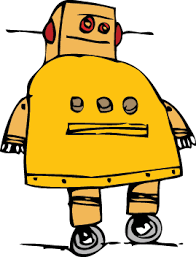
\includegraphics[width=100pt,height=100pt]{Déroulé/Jour_1/logo_instructables.png}\\
        \caption[Sites de modèles 3D]{Logos de quelques sites de modèles 3D}
        \label{fig:my_label}
        \end{center}
    \end{figure}
    
    
    \vskip0.5cm
    \begin{tabular}{|l|l|}
        \hline Site & Lien\\
        \hline Grabcad & \url{https://grabcad.com/library}\\
        \hline Cults3D & \url{https://grabcad.com/library}\\
        \hline Thingiverse & \url{https://www.thingiverse.com/}\\
        \hline Instructables & \url{https://www.instructables.com/workshop/3d-printing/projects/}\\
        \hline
    \end{tabular}\\\vskip0.5cm
    \href{https://all3dp.com/fr/1/ficher-stl-3d-gratuit-modele-3d-imprimante-3d/}{Ici}, le lien d'un article répertoriant plus de plateformes pour trouver des fichiers 3D.\\\vspace{0.2cm}
    
    \begin{multicols}{2}
    
\includegraphics[width=60pt,height=60pt]{Déroulé/Jour_1/Manuel d'utilisation/Images/6.jpg}
    
    \columnbreak
    
    \textbf{\large Attention : }\textbf{\textit{\large Certains de ces sites nécessitent la création d'un compte pour pouvoir télécharger les modèles, et certains modèles peuvent être payants.}}
    \end{multicols}
\end{flushleft}

\begin{flushleft}
    Trouver son modèle c'est bien... L'imprimer c'est mieux ! \textbf{Mais comment faire pour imprimer son fichier 3D ?}\\
    Pour pouvoir effectuer une impression 3D il faut passer via un logiciel dit "Trancheur 3D" (ou Slicer 3D en anglais).\vspace{0.4cm}
    
    \textbf{Mais qu'est-ce qu'un trancheur 3D ?}\\
    Un trancheur permet de calculer les couches qui seront imprimées ce qui revient à découper l'objet en intervalles de hauteur réguliers. De nombreux paramètres peuvent être ajustés afin d'adapter l'impression à l'imprimante 3D et à la qualité souhaitée de l'objet. Ils sont généralement identiques d'un logiciel à l'autre, nous les aborderons donc lors de la prise en main d'\textit{Ultimaker Cura}.
    
    \href{https://all3dp.com/fr/1/meilleur-slicer-3d-logiciel-decoupe-impression-3d/}{Ici}, le lien d'un article regroupant les trancheurs 3D utilisés le plus couramment.\\\vspace{0.2cm}
    
    \begin{multicols}{2}
    
\includegraphics[width=60pt,height=60pt]{Déroulé/Jour_1/Manuel d'utilisation/Images/6.jpg}
    
    \columnbreak
    
    \textbf{\large Attention : }\textbf{\textit{\large Certains de ces logiciels possèdent différentes versions. Certaines gratuites, d'autres payantes.}}
    \end{multicols}
\end{flushleft}

\subsubsection{Ce que l'on utilise pour cet atelier}
\begin{multicols}{2}
    
\includegraphics[width=50pt,height=50pt]{Déroulé/Jour_1/logo_cura.png}\\
    \columnbreak
    \begin{flushleft}
        Au cours de cet atelier, nous allons uniquement utiliser le logiciel \textit{Ultimaker Cura} pour visualiser puis imprimer les différentes pièces de la main.
    \end{flushleft}
\end{multicols}

%provisoire
\newpage

\begin{flushleft}
    \textbf{La source des fichiers utilisés pour imprimer la main :}
    
    Toutes les pièces 3D que nous utilisons viennent du projet de \href{https://www.instructables.com/3D-Printed-Robotic-Hand/}{TechMartian} (cliquer sur le pseudo pour accéder à la page de son projet et aux fichiers d'impression 3D) et sont également disponibles sur le site de \href{https://www.association-robots.com/}{\textit{Robots!}}. Ci-dessous, une photographie du modèle final qu'il a réalisé :\\
    
    \begin{figure}[!h]
        \centering
        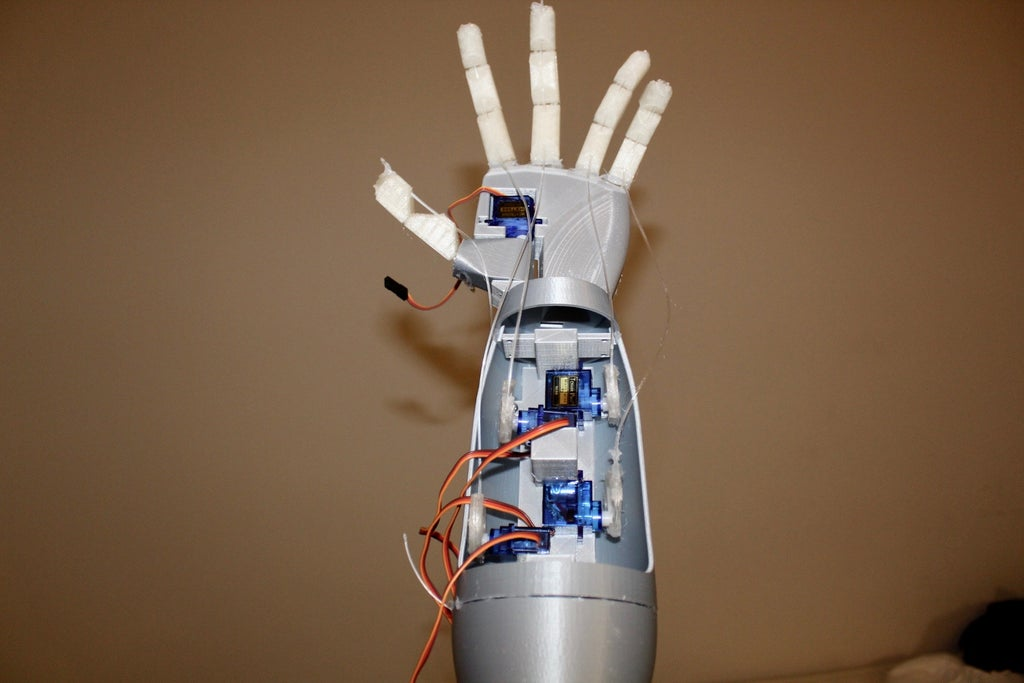
\includegraphics[width=200pt]{Déroulé/Jour_1/modèle_choisi.jpg}
        \caption[Projet de TechMartian]{Main robotique réalisée par TechMartian}
        \label{fig:my_label}
    \end{figure}
\end{flushleft}

\begin{flushleft}
     Au cours de l'atelier nous allons pas à pas monter et programmer notre modèle.
     Ci-dessous, une photo du modèle auquel nous arriverons à la fin de l'atelier:\\
    
    \begin{figure}[!h]
        \centering
        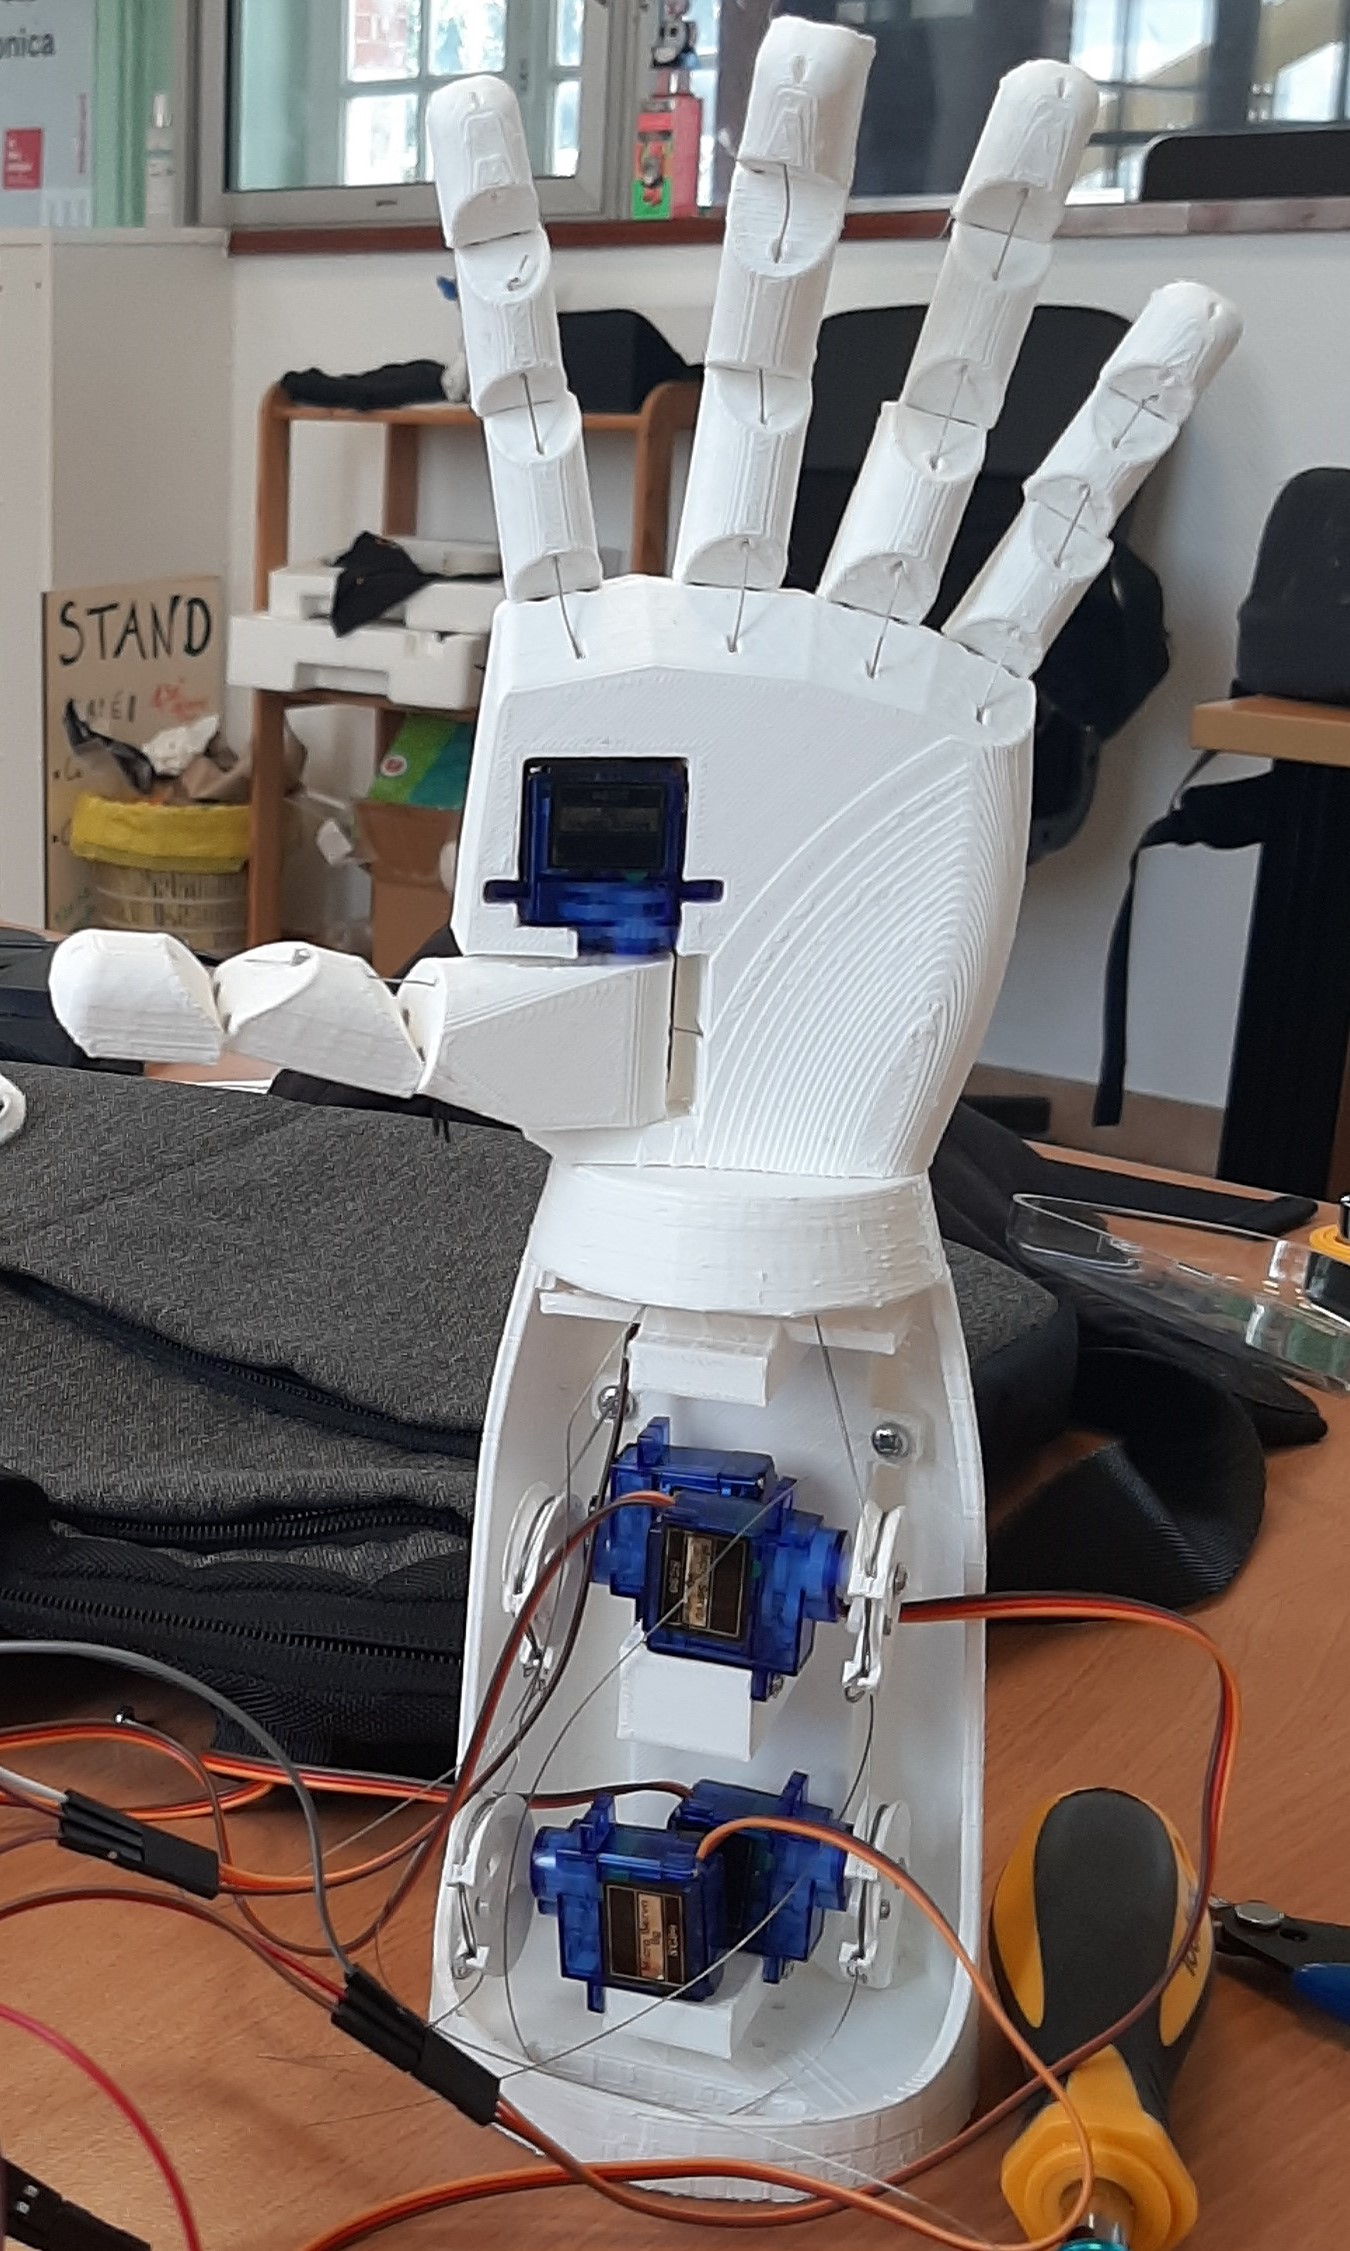
\includegraphics[width=200pt]{Déroulé/Jour_1/notre_version.jpg}
        \caption[Notre main]{Main robotique réalisée durant l'atelier}
        \label{fig:my_label}
    \end{figure}
\end{flushleft}

%provisoire
\newpage

\subsection{Où réaliser ses propres impressions 3D ?}

\begin{flushleft}
Vous n'avez pas d'imprimante 3D à la maison? Pas de problème !\vspace{0.2cm}

\textbf{À Nantes :}

\vspace{0.2cm}
\textbullet \, Contacter la société \href{https://dulse.fr/}{\textit{Dulse}}, membre du collectif \href{https://makeici.org/location-ateliers/nantes/}{\textit{Ici Nantes}} pour réaliser vos impressions. Le collectif propose également des formations certifiantes en impression 3D. (cliquer sur Ici Nantes pour avoir accès à leur catalogue de formations)\vspace{0.2cm}

\textbf{\large Note : }\textbf{\textit{\large Ces formations sont payantes mais sont éligibles au CPF (Compte Personnel de Formation).}}\vspace{0.2cm}

\textbullet \, Se rendre au FabLab de l'association \href{https://info.pingbase.net/faire-ensemble/#1598359300657-bc519d81-3b9f}{\textit{PiNG}}.\vspace{0.2cm}

\begin{multicols}{2}
    
\includegraphics[width=75pt,height=75pt]{Déroulé/Jour_1/Manuel d'utilisation/Images/6.jpg}
    
    \columnbreak
    
\textbf{Attention : }\textbf{\textit{Avant de pouvoir réaliser vos propres impressions sur les machines du FabLab, il vous faudra adhérer à PiNG. Renseignez vous sur leur site pour voir les offres proposées.}}\\
\end{multicols}
\end{flushleft}

\begin{flushleft}
\textbf{De manière un peu plus générale :}\\
\textbullet \vspace{2mm} Le \textit{pôle EMC2} a développé le site \href{https://meet3d.fr/imprimante/list}{\textit{Meet3D}}, qui recense les ressources en impression 3D.\vspace{0.2cm}

\textbullet \vspace{2mm} Il existe également une carte des FabLabs réalisée par le site \textit{Makery.info}.

\begin{figure}[!h]
    \centering
    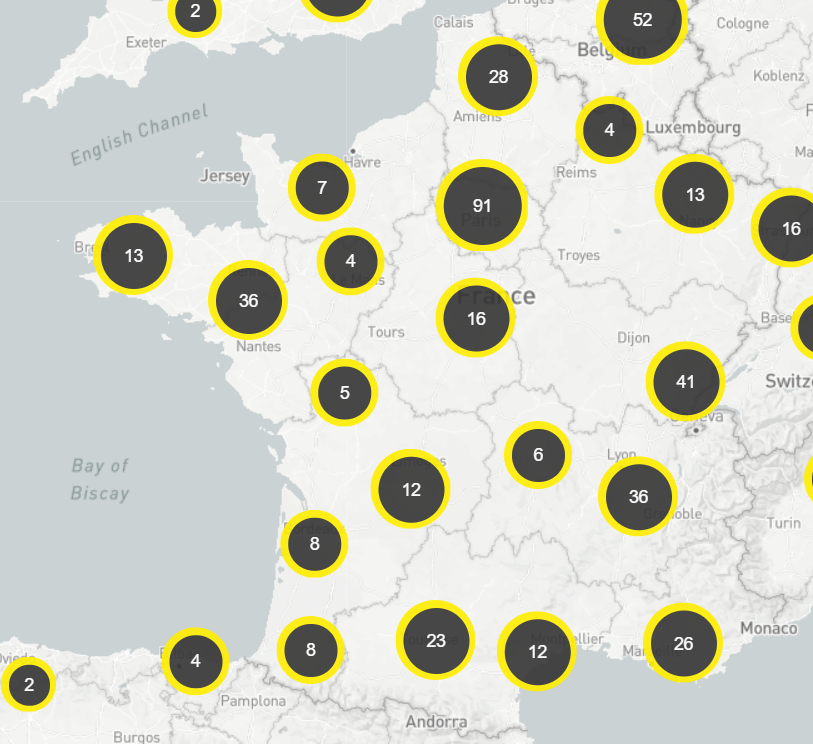
\includegraphics[width=250pt,height=250pt]{Déroulé/Jour_1/Carte_des_FabLab_France.PNG}
    \caption[Carte des FabLabs]{Carte de France des FabLabs}
    \label{fig:my_label}
\end{figure}
La carte détaillée avec les adresses est disponible \href{https://www.makery.info/labs-map/}{ici}.
\end{flushleft}

%provisoire
\newpage

\subsection{Utilisation de l'imprimante 3D}

\subsubsection{Notions de sécurité}

\begin{multicols}{2}


\includegraphics[width=50pt]{Déroulé/Jour_1/Manuel d'utilisation/Images/6.jpg}\\

\columnbreak
\begin{flushleft}
La buse et le plateau chauffent pendant l'utilisation. Attendre que l'imprimante ait refroidi avant d'essayer d'enlever les pièces ou les résidus de filaments.\\
\end{flushleft}

\end{multicols}

\begin{multicols}{2}


\includegraphics[]{Déroulé/Jour_1/Manuel d'utilisation/Images/1.PNG}\\

\columnbreak
\begin{flushleft}
L’imprimante présente des parties mobiles pouvant être dangereuses.
Ne pas toucher la machine pendant son fonctionnement.\\
\end{flushleft}

\end{multicols}

\begin{multicols}{2}


\includegraphics[]{Déroulé/Jour_1/Manuel d'utilisation/Images/5.PNG}\\

\columnbreak
\begin{flushleft}
Ne pas laisser l'imprimante à la portée des enfants.
\end{flushleft}

\end{multicols}

\begin{multicols}{2}

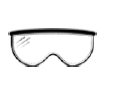
\includegraphics[]{Déroulé/Jour_1/Manuel d'utilisation/Images/2.PNG}\\

\columnbreak
\begin{flushleft}
Il est recommmandé d'utiliser des lunettes de protection lorsque l'on nettoie les pièces pour éviter que des projections entre en contact avec les yeux.\\
\end{flushleft}

\end{multicols}

\begin{multicols}{2}


\includegraphics[]{Déroulé/Jour_1/Manuel d'utilisation/Images/3.PNG}\\

\columnbreak
\begin{flushleft}
Ne pas rester trop proche de l'imprimante pendant l'impression, les vapeurs peuvent être dangereuses. Utiliser si possible l'imprimante dans une pièce aérée ou ventilée.
\end{flushleft}

\end{multicols}

\begin{multicols}{2}


\includegraphics[]{Déroulé/Jour_1/Manuel d'utilisation/Images/4.PNG}\\

\columnbreak
\begin{flushleft}
Ne pas mettre d'eau sur l'imprimante.
\end{flushleft}

\end{multicols}

%provisoire
\newpage

\subsubsection{Prise en main du logiciel \textit{Ultimaker Cura}}

\begin{flushleft}
\textbf{Installation du logiciel :}\vskip0.4cm

\textbullet \, Se rendre sur le site : \url{https://ultimaker.com/fr/software/ultimaker-cura}\vspace{0.2cm}

\textbullet \vspace{2mm} Aller dans la section \textit{Logiciel} :
\begin{figure}[!h]
    \centering
    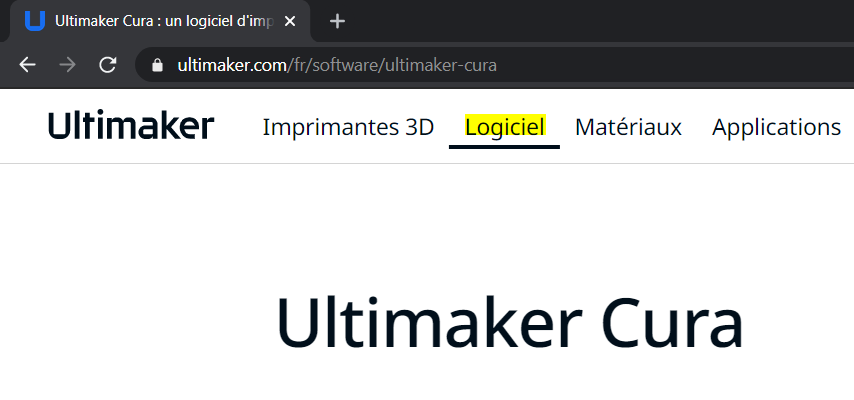
\includegraphics[width=400pt]{Déroulé/Jour_1/étape1.PNG}
    \caption{Installation Cura - \'Etape 1}
    \label{fig:my_label}
\end{figure}

\textbullet \, Descendre jusqu'à \textit{Ultimaker Cura} et cliquer sur \textit{En savoir plus} :
\begin{figure}[!h]
    \centering
    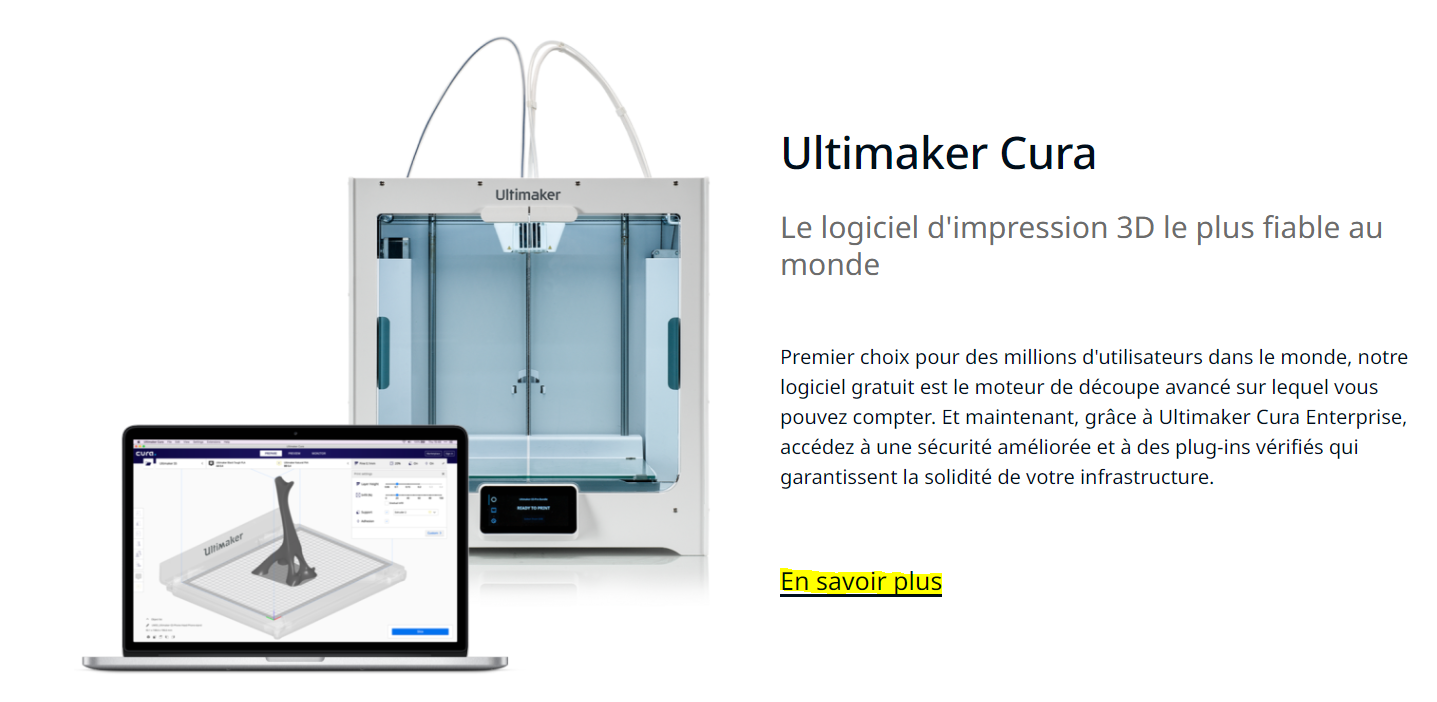
\includegraphics[width=400pt]{Déroulé/Jour_1/étape2.PNG}
    \caption[\'Etape 2]{Installation Cura - \'Etape 2}
    \label{fig:my_label}
\end{figure}

%provisoire
\newpage

\textbullet \, Cliquer sur \textit{Télécharger gratuitement} :
\begin{figure}[!h]
    \centering
    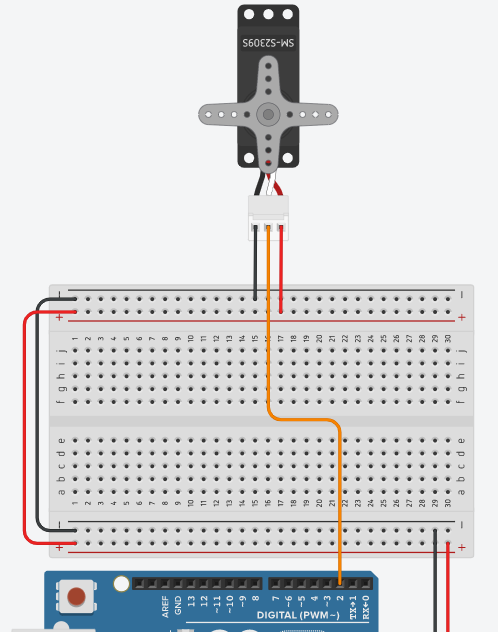
\includegraphics[width=300pt]{Déroulé/Jour_1/étape3.PNG}
    \caption[\'Etape 3]{Installation Cura - \'Etape 3}
    \label{fig:my_label}
\end{figure}
\end{flushleft}

\begin{flushleft}
\textbf{Configuration du logiciel :}\vspace{0.4cm}

\textbullet \, Cliquer sur la petite flèche :
\begin{figure}[!h]
    \centering
    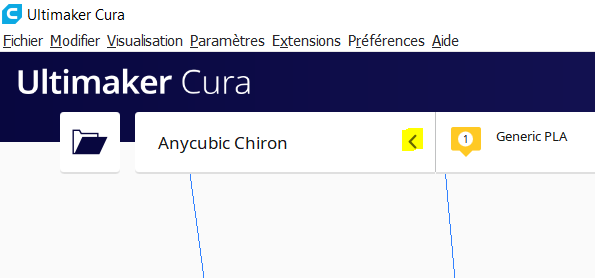
\includegraphics[width=300pt]{Déroulé/Jour_1/réglagesCura_étape1.PNG}
    \caption{Configuration Cura - \'Etape 1}
    \label{fig:my_label}
\end{figure}

%provisoire
\newpage

\textbullet \, Cliquer sur \textit{ajouter une imprimante} :
\begin{figure}[!h]
    \centering
    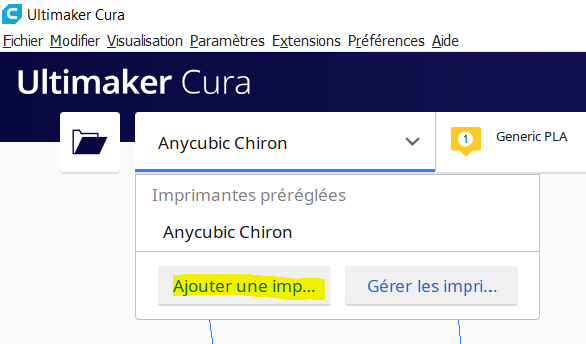
\includegraphics[width=300pt]{Déroulé/Jour_1/réglagesCura_étape2.PNG}
    \caption[\'Etape 2]{Configuration Cura - \'Etape 2}
    \label{fig:my_label}
\end{figure}

\textbullet \, Choisir son imprimante en réseau si elle est disponible, ou la sélectionner manuellement en allant dans \textit{hors réseau} sinon, puis l'ajouter :
\begin{figure}[!h]
    \centering
    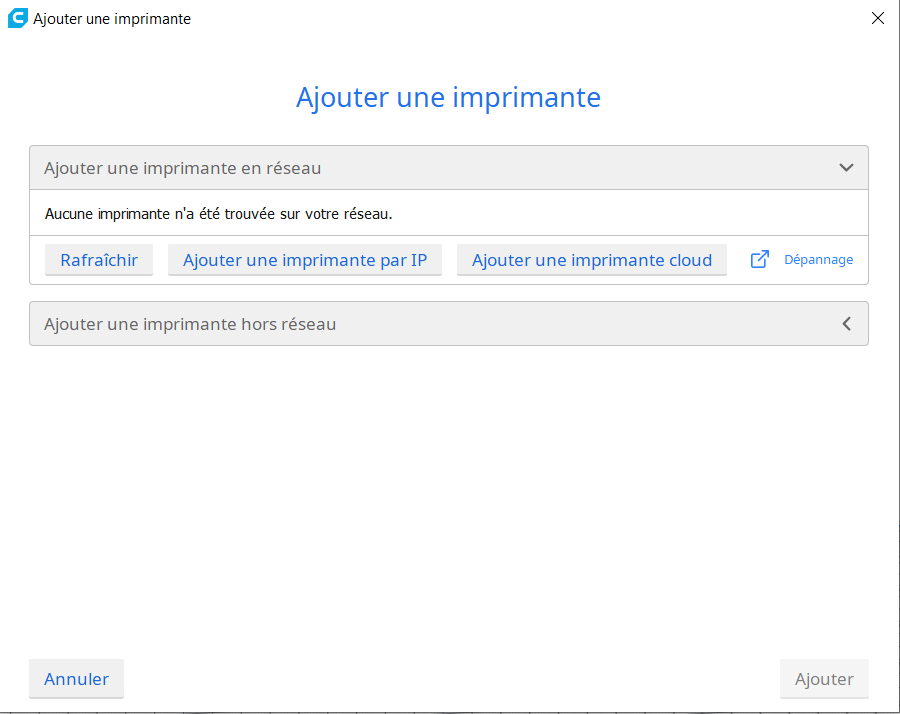
\includegraphics[width=300pt]{Déroulé/Jour_1/réglagesCura_étape3.PNG}
    \caption[\'Etape 3]{Configuration Cura - \'Etape 3}
    \label{fig:my_label}
\end{figure}

%provisoire
\newpage

\textbullet \, Cliquer sur la petite flèche pour choisir le type de filament que vous allez utiliser :
\begin{figure}[!h]
    \centering
    
\includegraphics[width=300pt]{Déroulé/Jour_1/réglagesCura_étape4.PNG}
    \caption[\'Etape 4]{Configuration Cura - \'Etape 4}
    \label{fig:my_label}
\end{figure}

\textbullet \, Cliquer sur le petit crayon pour régler les paramètres d'impression :
\begin{figure}[!h]
    \centering
    
\includegraphics[width=300pt]{Déroulé/Jour_1/réglagesCura_étape5.PNG}
    \caption[\'Etape 5]{Configuration Cura - \'Etape 5}
    \label{fig:my_label}
\end{figure}

\textbullet \, Modifier les paramètres d'impression comme suit :\\
\begin{figure}[!h]
    \centering
    \begin{tabular}{|l|l|l|}
    
    \hline Catégorie & Nom du paramètre & Valeur\\
    \hline Qualité & Hauteur de la couche & 0.3 mm\\
    \hline Coque & \'Epaisseur de la paroi & 0.5 mm\\
    \hline & Nombre de lignes de la paroi & 1\\
    \hline & \'Epaisseur du dessus/dessous & 0.8 mm\\
    \hline & \'Epaisseur du dessus & 0.8 mm\\
    \hline & Couche supérieure & 3\\
    \hline & \'Epaisseur du dessous & 0.8 mm\\
    \hline & Couche inférieure & 3\\
    \hline & Expansion horizontale & 0 mm\\
    \hline Remplissage & Densité du remplissage & 17.5\% \\
    \hline & Motif de remplissage & Grille\\
    \hline Matériau & Température d'impression & 200°C\\
    \hline & Température du plateau & 85°C\\
    \hline Vitesse & Vitesse d'impression & 80mm/s\\
    \hline Déplacement & Activer la rétraction & Oui\\
    \hline Refroidissement & Activer le refroidissement de l'impression & Oui\\
    \hline & Vitesse du ventilateur & 100\% \\
    \hline Supports & Générer les supports & Non \\
    \hline Adhérence du plateau & Type d'adhérence du plateau & Bordure \\
    \hline 
    
    \end{tabular}
    \caption[\'Etape 6]{Configuration Cura - \'Etape 6}
    \label{fig:my_label}
\end{figure}

\begin{multicols}{2}
    
\includegraphics[width=60pt,height=60pt]{Déroulé/Jour_1/Manuel d'utilisation/Images/6.jpg}
    
    \columnbreak
    
\textbf{\large Attention : }\textbf{\textit{L'imprimante que nous avons utilisé pour le projet est une Chiron de chez Anycubic, et le type filament utilisé est le PLA. Les paramètres d'impression seront peut-être à régler différemment si vous utilisez une autre imprimante et un autre type de filament.}}\\\vspace{0.2cm}
\end{multicols}

\textbullet \, Aller dans \textit{fichier} puis \textit{Ouvrir le(s) fichier(s)} et sélectionner celui que vous voulez imprimer :
\begin{figure}[!h]
    \centering
    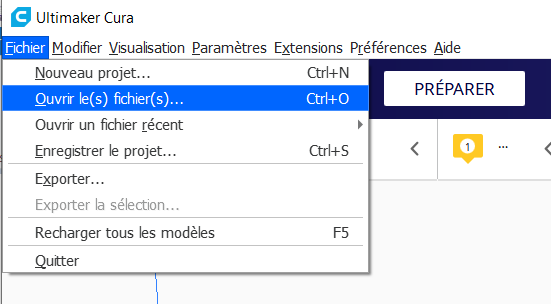
\includegraphics[width=300pt]{Déroulé/Jour_1/réglagesCura_étape7.PNG}
    \caption[\'Etape 7]{Configuration Cura - \'Etape 7}
    \label{fig:my_label}
\end{figure}


\includegraphics[width=30pt,height=30pt]{Déroulé/Jour_1/idée.png}
\textbf{\large Astuce : }\textbf{\textit{\large Si le plateau de votre imprimante est assez grand, il est possible d'imprimer plusieurs pièces simultanément. Pour cela il faut les positionner de part et d'autre du plateau virtuel sur Cura. Pour ce faire, cliquez sur la pièce que vous voulez déplacer et bouger la en restant appuyé sur la flèche correspondant à la direction souhaitée.}}\\\vspace{0.2cm}


\includegraphics[width=30pt,height=30pt]{Déroulé/Jour_1/idée.png}
\textbf{\large Astuce : }\textbf{\textit{\large La température de la pièce dans laquelle vous êtes influe également sur la qualité de votre impression.}}\\
\end{flushleft}

\newpage